
\chapter{Sistemi anti-DDoS: stato dell'arte}
% attacchi e contromisure sui ddos

% Quando Internet è stato inventato non si pensava a questo problema e non sono state implementate difese
\section{Gli attacchi DDoS}

Gli attacchi di Denial of Service (DoS) sono attacchi nel campo della sicurezza informatica che mirano a interrompere la fruizione di un servizio, fornito da un host connesso a internet, da parte di utenti legittimi. L'attacco ha l'obiettivo di esaurire le risorse dell'host in modo da non consentirgli di erogare le risposte ai richiedenti.
Nel caso in cui la sorgente del traffico che genera traffico malevolo per creare disservizi non sia unica, si parla di attacchi di denial of service distribuiti (Distributed Denial of Service).

\subsection{Tipologia di attacchi DDoS}
    
Gli attacchi DDoS possono essere suddivisi in due categorie principali in base al loro funzionamento. La prima si basa sul mandare alla vittima pacchetti malformati in grado di sfruttare un bug o una falla a livello applicativo. La seconda categoria invece si basa su tecniche utili a colpire l'infrastruttura del servizio, per il funzionamento di questa tecnica vengono usati uno o entrambi i seguenti metodi: il primo si basa sull'interruzione della connessione di rete grazie all'esaurimento della banda o della capacità di processamento dei router o di entrambe, nel secondo caso l'obiettivo dell'attaccante è di esaurire le risorse (es. sockets, CPU, memoria) del server che ospita il servizio \cite{ddos_survey_1}.

\begin{figure}[h]

    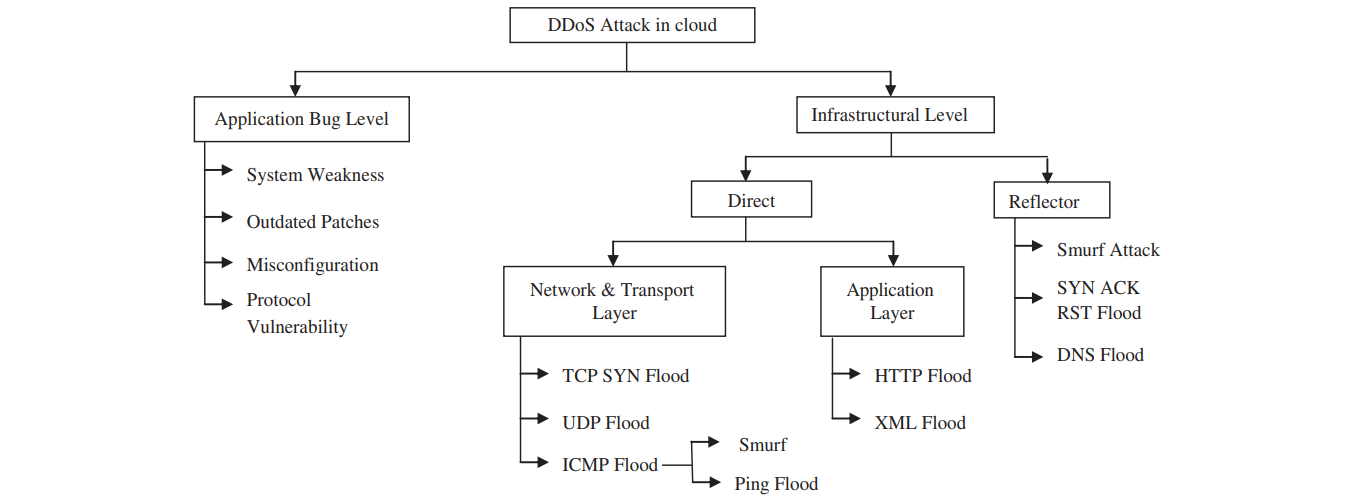
\includegraphics[width=\hsize]{images/introduzione/tipologie_ddos.png}
    \caption{Tipologie di attacchi DDoS \cite{ddos_survey_3}}
    \centering
\end{figure}

L'obiettivo di questa tesi sarà concentrato sul rilevamento e la mitigazione della seconda categoria di attacchi, basata sull'esaurimento delle risorse.

\subsubsection{Attacchi basati sul flooding}

\begin{figure}[h]
    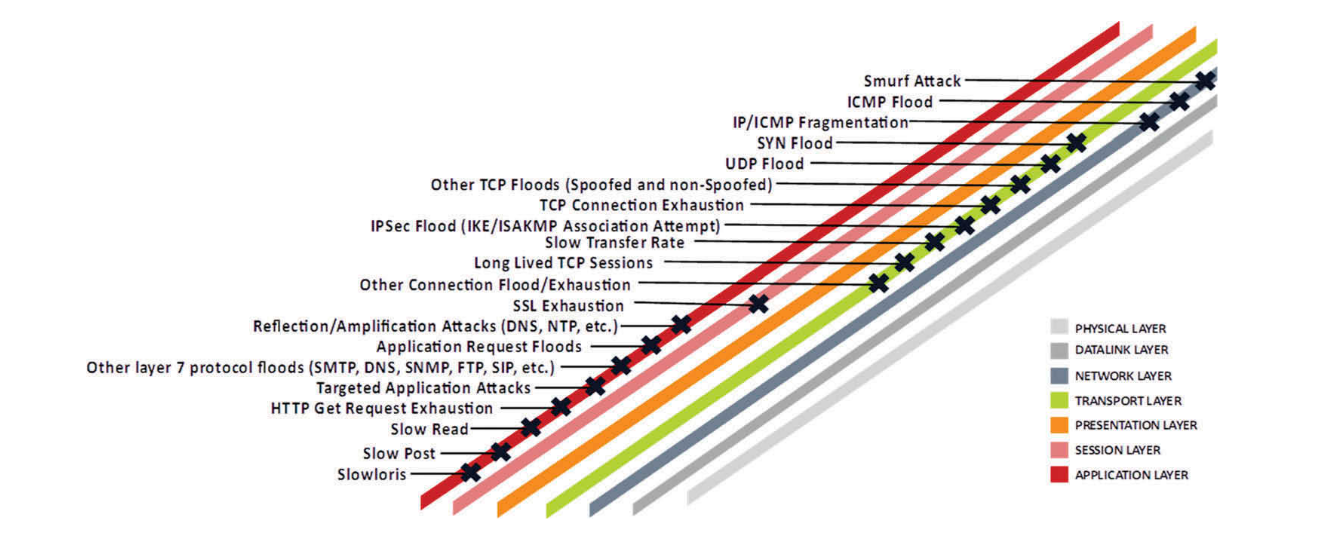
\includegraphics[width=\hsize]{images/introduzione/attacchi_per_livello.png}
    \caption{Attacchi per livello \cite{ddos_survey_4}}
    \centering
\end{figure}

\paragraph{Network/transport-level DDoS flooding attacks} % todo: rivedere titolo
Gli attacchi di denial of service che mirano ad esaurire le risorse di rete si basano sull'invio di molti pacchetti con lo scopo di consumare totalmente la banda o le strutture dati relative al livello di trasporto della vittima, queste tipologia di attacco può essere effettuata in maniera diretta: \emph{flooding attacks} e \emph{protocol exploitation attacks}, nel primo caso la vittima viene inondata di pacchetti (UDP flood, ICMP flood, DNS flood, VoIP flood, etc.), in questo caso la banda aggregata in uscita di tutti gli attaccanti deve essere superiore a quella del servizio che si vuole danneggiare. Nel secondo caso vengono sfruttane delle caratteristiche dei protocolli della vittima in modo da consumare una grande quantità di risorse (es. TCP SYN flood, TCP SYN-ACK flood, RST/FIN flood e ecc) utilizzando una minore quantità di banda.

Gli attacchi che non vengono effettuati in maniera diretta invece sfruttano la riflessione o l'amplificazione: nei \emph{Reflection-based flooding attacks} chi attacca manda un particolare pacchetto, indirizzandolo ad un riflettore e questo riflettore manda le sue risposte alla vittima, in modo da esaurirne le risorse. Un esempio di questa tipologia di attacchi sono lo Smurf e il Fraggle, nel primo vengono mandati ICMP Echo Request ad una sottorete, utilizzando l'ip spoofing per mandare pacchetti, con ip di destinazione l'indirizzo broadcast e specificando come ip sorgente l'ip della vittima, questa tecnica provocherà la risposta di tutti gli host verso l'indirizzo IP della vittima usato come sorgente \cite{ddos_survey_2}.
Gli \emph{Amplification-based flooding attacks} sfruttano servizi che restituiscono risposte più grandi della richiesta ricevuta, un esempio è il DNS amplification, che riesce a moltiplicare dalle 30 alle 50 volte \cite{imperva_amplification} la banda in uscita dell'attaccante, il suo funzionamento si basa sull'utilizzo dell'ip spoofing mandando un pacchetto con indirizzo ip sorgente della vittima, così il servizio DNS risponderà ad essa con un flood di pacchetti di dimensioni maggiori \cite{ddos_survey_1}. Lo stesso principio è sfruttato anche dal NTP amplification che può aumentare il traffico con un rapporto tra 20:1 e 200:1, arrivando in alcuni casi anche a 556:1 \cite{imperva_amplification}. 

% todo: Amplification-based flooding attack, negli attacchi di rete: qua non so giustificarla bene pagina 3 \cite{ddos_survey_1}
% qua parla bene del fattore di moltiplicazione degli attacchi https://www.imperva.com/blog/ntp-flood-explained/

\paragraph{Application-level DDoS flooding attacks} % todo: rivedere titolo
% qua taglio un po' corto sugli attacchi applicativi perché approfondirò maggiormente quelli di rete
Gli attacchi DDoS al livello applicativo hanno lo scopo di terminare le risorse del server(cpu, memory, disk/db bandwidth, I/O bandwidth), solitamente usano meno banda rispetto gli attacchi rivolti verso l'infrastruttura di rete rete, per questo motivo è anche più difficile identificarli. Le tecniche utilizzate sono simili alle precedenti. Degli esempi sono l'HTTP flooding che effettuando l'invio di molte richieste HTTP, obbliga il server a produrre risposte che possono essere computazionalmente pesanti, oppure possono sfruttare l'SQL Injection per imporre un lock sul database e bloccare il funzionamento dell'applicazione. Altri attacchi di questa tipologia possono essere l'HTTP fragmentation, lo slowpost attack, slowreading attack e lo slowloris attack, tutte tecniche che mirano a mantenere molte connessioni aperte mandando o ricevendo pochi dati per volta \cite{ddos_survey_1}.
Gli attacchi di tipo applicativo sono molto eterogenei e non possono essere mitigati a livello di rete/trasporto, per questo motivo questa tesi prenderà in considerazione solo gli attacchi trattati al paragrafo precedente.

\paragraph{DDoS con obiettivo la riduzione della qualità del servizio}
\label{paragraph:ddos_degradation}
% parlare anche di attacchi a basso rate, ma da molte fonti che portano ad un grande risultato finale \cite{ddos_survey_4,ddos_survey_3} pagina 38, rendendolo difficile da indentificare

L'unico obiettivo possibile degli attacchi DDoS non è la sola interruzione del servizio. Un altro risultato attuabile è la degradazione del servizio, consumando una parte di risorse destinate agli utenti legittimi e creando loro ritardi nelle risposte. Questo risultato può essere raggiunto utilizzando dei packet rate più bassi, e di conseguenza meno rilevabili o dei l'invio di flood di pacchetti con rate variabili \cite{ddos_survey_3, ddos_survey_4}.
Gli approcci a bassi rate sono utilizzati frequentemente dagli attacchi DDoS su larga scala, poiché l'aggregazione di moltissime fonti a basso rate portano comunque ad un grande risultato finale.

\subsection{Vittime attacchi DDoS}

% todo: introduzione: qua potrei nominare delle statistiche sugli attacchi con la distribuzione delle vittime
\begin{figure}[h]
    % todo: capire come gestire citazioni immagini a livello di copyright
    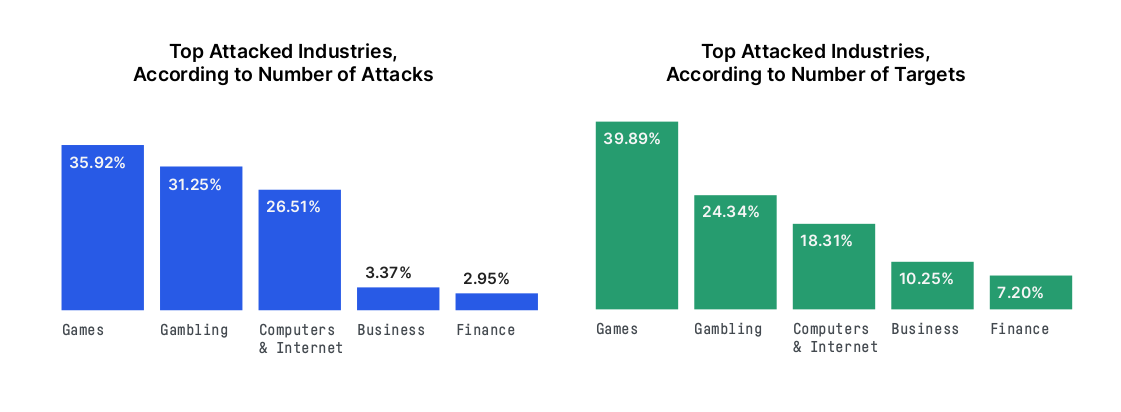
\includegraphics[width=\hsize]{images/introduzione/bersagli_ddos.png}
    \caption{Distribuzione vittime DDoS, 2020 \cite{imperva_ddos_report}}.
    \centering
\end{figure}

I target degli attacchi DDoS possono differenziarsi molto: da un utente domestico ad un governo \cite{ddos_motivations}. Per capire maggiormente chi possono essere le vittime di un attacco bisogna analizzare le motivazioni che spingono gli attaccanti e con le diverse motivazioni si può anche capire qual'è il rischio per quanto riguarda la portata dell'attacco. 

Per semplicità possiamo suddividere gli incentivi di un attacco in cinque principali categorie \cite{ddos_survey_1, ddos_motivations}:

\begin{itemize}
    \item Beneficio economico o finanziario: sono gli attacchi riguardanti principalmente le aziende, sono considerati i più pericolosi e difficili da fermare. Mirano ad ottenere benefici finanziari dagli attacchi e i creatori dell'attacco sono abitualmente persone con esperienza.
    \item Vendetta: questa tipologia di attacchi sono mesi in atto da persone, solitamente con uno scarso livello tecnico, a fronte di un'apparente ingiustizia percepita.
    \item Credo ideologico: alcuni attaccanti si trovano ad effettuare attacchi contro alcuni obiettivi per motivi ideologici. È una motivazione di attacco meno comune delle altre, ma può portare ad attacchi di grande entità. % todo: valutare se mettere esempi attacchi tipo cnn 2008, wikileaks 2010 e iran 2009
    \item Sfida intellettuale: gli utenti che sviluppano attacchi per questa motivazione vogliono imparare e sperimentare a lanciarli. Spesso sono giovani appassionati di hacking che grazie alla facilità con cui si possono affittare botnets o utilizzare semplici tool riescono ad effettuare con successo DDoS.
    \item Cyberwarfare: gli attaccanti di questa categoria appartengono ad organizzazioni terroristiche o militari di un paese e sono politicamente motivati ad attaccare risorse critiche di un altro paese. Un grande numero di risorse viene usato per questa tipologia di attacco e può paralizzare le infrastrutture critiche di un paese, portando ad un grave impatto economico.
\end{itemize}


Le maggiori vittime secondo il report \cite{imperva_ddos_report} sono le compagnie che operano del campo dei videogiochi e delle scommesse, entrambe comportano un grande livello di rischio e spesso i giocatori si rifiutano di seguire le regole. Le aziende che incentrano il loro business sul settore di Internet e della computazione si trovano al terzo posto, seguiti dalle attività commerciali e da quelle finanziarie.


\subsection{Diffusione attacchi DDoS}


\begin{figure}[h]
    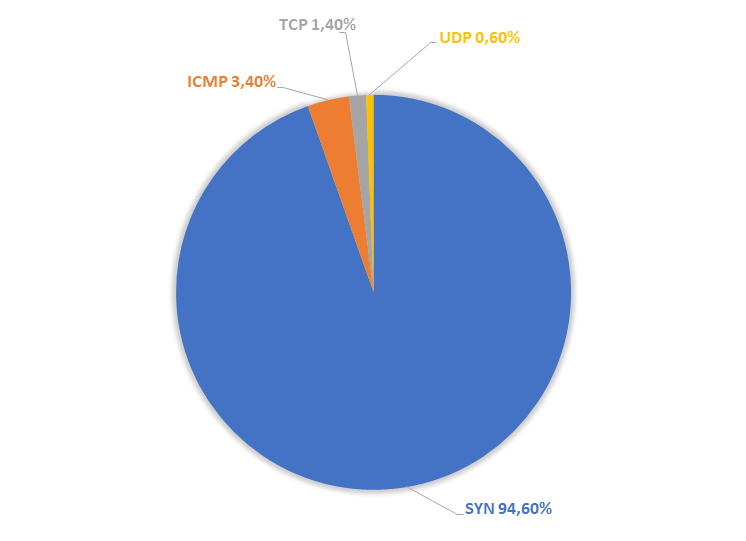
\includegraphics[width=\hsize]{images/introduzione/tesi_distribuzione_tipologia_attacchi.png}
    \caption{Distribuzione di attacchi DDoS per tipologia, Q3 2020 \cite{ddos_kaspersky_q3_2020}}
    \centering
\end{figure}

Nel mondo a fine 2020 la quasi totalità degli attacchi DDoS proviene da botnets, con target principali in Cina e negli Stati Uniti. Le tipologie di attacco maggiormente utilizzate sono il \emph{Syn Flood} che copre più del 90\% della totalità degli attacchi, seguito da \emph{ICMP flooding} e \emph{UDP flooding} \cite{ddos_kaspersky, ddos_kaspersky_q3_2020}.


La maggior parte degli attacchi DDoS hanno una portata inferiore ai 10 Gbps (circa il 65\%), ma il 3\% di essessi raggiunge cifre incredibili, superiori al 200 Mbps \cite{imperva_ddos_report}.

\begin{figure}[h]
    % todo: capire come gestire citazioni immagini a livello di copyright
    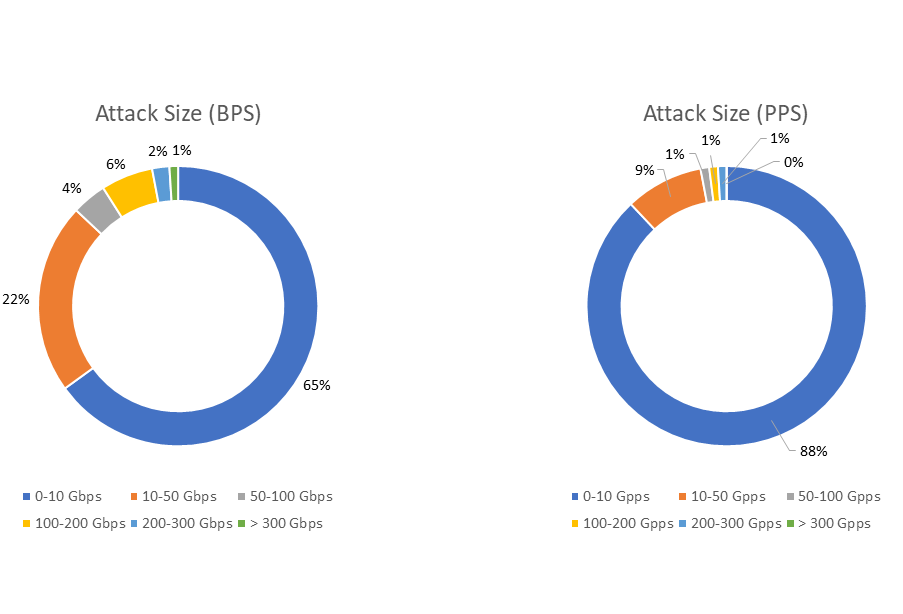
\includegraphics[width=\hsize]{images/introduzione/attacks_size_2.png}
    \caption{Distribuzione di attacchi DDoS per dimensione, 2020 \cite{imperva_ddos_report}}
    \centering
\end{figure}


\subsubsection{Attacchi basati su botnets}

Gli attacchi basati su botnets sono un grande problema per l'implementazione di sistemi anti-DDoS perché un grande numero di ``zombie'' rende l'attacco più distruttivo, in aggiunta spesso utilizzano ip spoofing complicando il tracciamento all'indietro per determinare la vera locazione dei bot \cite{ddos_survey_1}.

Il funzionamento delle botnet si basa su tre fasi. La prima consiste nel reclutamento ``dell'esercito'': fase in cui vengono contagiati i dispositivi tramite worms (programmi che si autopropagano) che sfruttano falle nella sicurezza. Sono usate tecniche come: la scansione automatica di indirizzi ip casuali per trovare altri soggetti vulnerabili, questa tipologia di scansione però produce molto traffico e può rendere possibile rilevare l'attacco, oppure una hitlist: una tecnica che frutta una lista di possibili macchine potenzialmente vulnerabili, la scansione della subnet o l'utilizzo di informazioni dei target basandosi sulle informazioni contenute nelle vittime infettate dai wormc.


% qui dovrei magari differenziare le botnet controllate direttamente e indirettamente e dilungarmi meno, magari nominare le tre fasi degli attacchi  \cite{ddos_motivations} pagina 5 \cite{ddos_survey_4} pagina 37
Nella fase successiva alla creazione di un ``esercito'' avviene la propagazione delle informazioni riguardanti le vittime da attaccare, con la durata e l'ora.
I bot possono essere controllati dell'artefice dell'attacco tramite tre architetture \cite{ddos_survey_4}: % pagina 46
\begin{itemize}
    \item IRC-based: architettura client-server in cui ad ogni server si possono collegare centinaia di dispositivi, utilizza un protocollo testuale e utilizzando porte non standard rendendo molto difficile il riconoscimento del comando per lanciare un DDoS, il quale si può nascondere facilmente nel grande traffico dei server IRC. Il singolo server a cui si connettono tutti i client può essere considerato un single point of failure.
    \item Web based: ogni bot scarica periodicamente delle informazioni tramite una richiesta web ad un server, i comandi di questa tipologia di controllo sono i più difficili da tracciare.
    \item P2P based: le moderne botnet utilizzano una struttura più robusta e flessibile, invece di avere un singolo server centrale al controllo della botnet, viene mandato un comando in broadcast a tutti gli agent. Questo le rende più affidabili, poiché l'eliminazione di un agent non rende la rete non funzionante, ma al tempo stesso rende il mantenimento della rete più difficile e la scoperta di un agent può rivelare tutti gli altri. 
\end{itemize}
L'ultima fase è il tentativo di attacco vero e proprio.

\begin{figure}[h]
    % todo: capire come gestire citazioni immagini a livello di copyright
    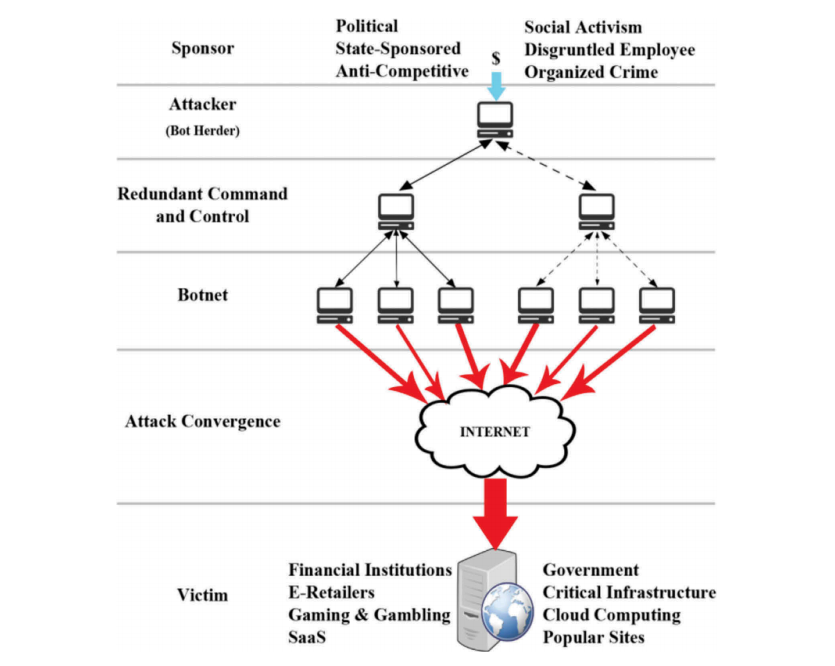
\includegraphics[width=\hsize]{images/introduzione/struttura_botnets_2.png}
    \caption{Struttura di lancio di attacchi DDoS \cite{ddos_survey_4}.}
    \centering
\end{figure}

Un esempio di botnet è Mirai, una rete di dispositivi creata attraverso un malware che sfrutta le vulnerabilità dei dispositivi IoT per creare host malevoli da utilizzare in attacchi DDoS di larga scala. Il codice sorgente del bot è stato rilasciato pubblicamente nel 2016, questo ha permesso la creazione di molte sue varianti, lasciando a chiunque la possibilità  di crearsi la propria botnet.
Il codice per effettuare attacchi DDoS include dieci tipologie diverse di attacco, ognuna configurabile in molti modi e lanciabile attraverso l'utilizzo di un server di comando e controllo \cite{slide_mirai}.

Alcuni attacchi possibili tramite la botnet Mirai sono: flood DNS, STOMP: una attacco che mira ad effettuare il three-way TCP handshake e solo dopo quando la sessione sarà messa in whitelist inizia un ACK flood, GREIP: incapsula nel pacchetto GRE un pacchetto ip con ip sorgente e destinazioni casuali, SYN flood, ACK flood, UDP flood e HTTP flood.

% \subsubsection{Attacchi DDoS famosi}

% %todo: qua parla del flood dns https://www.cloudflare.com/it-it/learning/ddos/dns-flood-ddos-attack/

% \uline{Aggiungo questa parte o sarebbe superflua?

% Potrei parlare dei primi attacchi, fino a quelli moderni menzionando i motivi dell'attacco se scoperti, la tipologia e la portata.}


\section{Riconoscimento DDoS}

% \cite{ddos_motivations} pagina 16, \cite{ddos_survey_4} pagina 66
La fase di riconoscimento degli attacchi DDoS è un importante passo per permettere la successiva mitigazione, questa fase diventa più facile maggiormente ci avviciniamo alla vittima dell'attacco, ma viceversa più ci si allontana dalla sorgente dell'attacco e più diventa difficile identificarla. In letteratura esistono due tecniche per identificare i flussi malevoli: signature-based detection e anomaly-based detection.

\subsection{Signature-based detection}

La signature-based detection è un meccanismo che si basa sul riconoscimento di attacchi DDoS conosciuti, differenziando la loro firma dai normali flussi della rete. Queste soluzioni hanno un buon successo con attacchi DDoS noti, ma non sono in grado di rilevare nuove tipologie di attacco delle quali non si conosce ancora la signature. Questi sistemi si possono basare su pattern matching (es. Bro/Zeek), su regole (es. Snort, Suricata), sulla correlazione di informazioni di management sul traffico o sull'analisi spettrale.
% todo: rivedere le ultime due perché non so bene cosa siano

\subsection{Anomaly-based detection}

I sistemi basati sul rilevamento delle anomalie possono riconoscere anche attacchi non conosciuti, basandosi su delle soglie per differenziare il traffico normale da quello malevolo, ma la scelta dei limiti oltre i quali considerare il traffico anomalo è una grande sfida per questa tipologia di tecniche.
I metodi più diffusi si basano su metodi statistici, di data mining o intelligenze artificiali.

\section{Contromisure attacchi DDoS}

Gli attacchi DDoS si raggruppano ad imbuto dalle sorgenti verso la vittima, per questa ragione più si è vicini alla vittima e più l'attacco sarà facile da riconoscere, ma più difficile da mitigare. Per questa ragione le tecniche di mitigazione vengono suddivise in base al luogo in cui vengono azionate.

\begin{figure}[]
    % todo: capire come gestire citazioni imsmagini a livello di copyright
    \label{fig:classificazione_ddos}
    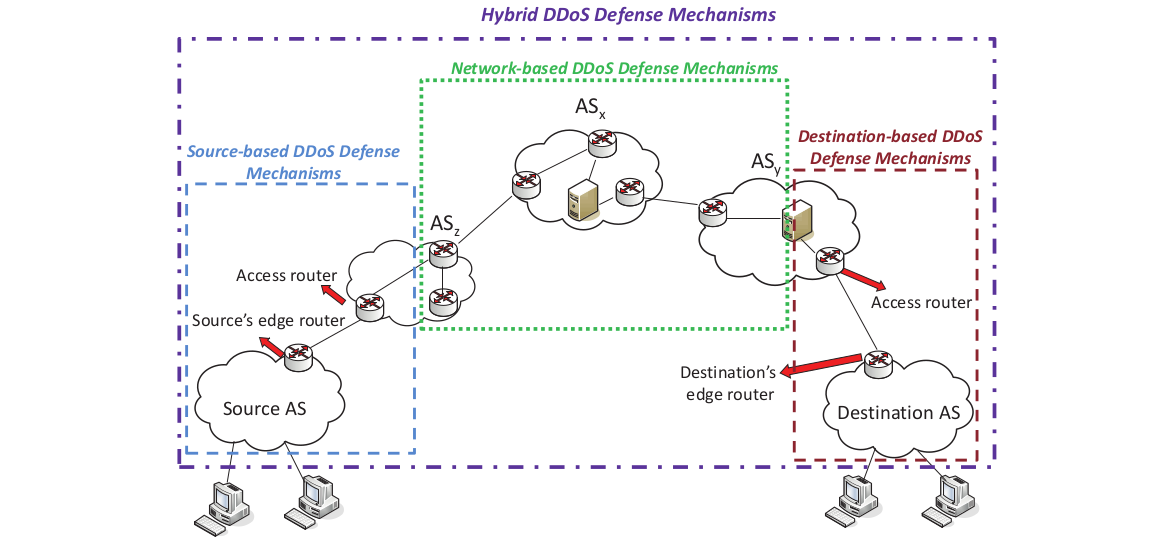
\includegraphics[width=\hsize]{images/ddos/classificazione_difese.png}
    \caption{Classificazione dei sistemi di difesa in base al luogo di applicazione \cite{ddos_survey_1}}
    \centering
\end{figure}

\subsection{Soluzioni alla sorgente}
Questa tipologia di soluzioni sono adottate vicino alle sorgenti dell'attacco per impedire agli utenti di una sottorete di generare attacchi DDoS. Queste soluzioni possono essere applicate agli edge router degli Autonomous System (AS) di accesso.

Degli esempi di soluzioni sono \cite{ddos_survey_1}:

% todo: completare elenco delle soluzioni alla sorgente
\begin{itemize}
    \item Filtri in ingresso e uscita agli edge router delle sorgenti: gli attacchi che si basano sulla riflessione sfruttano la tecnica dell'ip spoofing, lo scopo di questi filtri è di bloccare il traffico che lo utilizza senza interferire sul traffico legittimo.
    \item D-WARD: sistema che mira a rilevare attacchi di tipo DDoS flooding monitorando il traffico in ingresso e uscita e comparandolo con dei flussi normali di traffico. I flussi sono filtrati se non rispettano il modello. Per esempio può essere imposto un rapporto massimo tra pacchetti inviati e ricevuti per un flusso TCP che se superato può segnalare il flusso come anomalo.
    \item MULTOPS (MUlti-Level Tree for Online Packets Statistics): è un'euristica e un struttura dati che permette di rilevare attacchi provenienti da una subnet. Normalmente il traffico in una direzione è proporzionale a quello in quella opposta, una significativa differenza possono indicare che la rete è la sorgente o la vittima di un attacco DDoS.
    \item MANAnet’s Reverse Firewall: è un firewall che a differenza di quelli tradizionali, protegge l'esterno dal traffico in uscita dalla subnet.
\end{itemize}

I problemi di questa soluzione sono che per permettere una copertura totale, questi meccanismi dovrebbe essere implementatati su tutti gli edge router di tutti gli AS di accesso, inoltre è difficile differenziare il traffico legittimo, da quello malevolo e non meno importante non è chiaro chi sia il responsabile del mantenimento economico di questo servizio \cite{ddos_survey_1}.

\subsection{Soluzioni alla destinazione}

Esistono soluzioni che si possono applicare agli edge router della vittima, possono analizzare il suo comportamento, il suo traffico usuale e riconoscere le anomalie \cite{ddos_survey_1,ddos_survey_2}.
Delle soluzioni posizionate in questi luoghi possono essere dei proxy, firewall che gestiscono le connessioni semi aperte in caso di syn flood oppure l'utilizzo sistemi di tracciamento implementati in alcuni router (in caso di ip spoofing), per risalire alla vera sorgente dell'attacco e bloccarla. % todo: non so come concludere le soluzioni alla destinazione, sicuramente c'è qualche meccanismo che ho dimenticato \cite{ddos_survey_2, ddos_survey_1}

% todo: potrei descriverli in maniera più dettagliata 

Questi sistemi di difesa possono diventare i target degli attacchi, poiché spesso richiedono una grande quantità di memoria e potenza di processamento per effettuare le osservazioni delle misure statistiche \cite{ddos_survey_4}.

\subsection{Soluzioni sulla rete}

I sistemi anti-DDoS sulla rete si basano sui router o su firewall installati sulla rete dell'operatore.
Una prima soluzione adottata è quella del Router based packet filter, la quale si basa sui criteri dell'ingress filtering, ma applicandola ai router nel core della rete. Il traffico per ogni link tendenzialmente viene generato da un ristretto intervalli di indirizzi ip, quando appare un indirizzo ip sospetto viene filtrato, questa soluzione è adatta a rilevare attacchi che utilizzano ip spoofing, ma è inutile nel caso di utilizzo di ip genuini.
Altre soluzioni mirano ad identificare i router nel core di internet che sono stati compromessi e si comportano in modo anomalo, oppure mirano all'installazione di detection systems (DSs) i quali permettono di rilevare pattern anomali, ma sono computazionalmente molto dispendiosi.

I problemi di questa soluzione è l'introduzione di un overhead per il processamento sui router, inoltre il rilevamento degli attacchi è difficile a causa dei dati troppo poco aggregati.

\subsection{Soluzioni distribuite}

Le soluzioni distribuite creano una cooperazione tra i luoghi di installazione delle difese. Alla sorgente vengono installati i sistemi di difesa per filtrare l'attacco, mentre sulla rete della vittima ne viene effettuato il riconoscimento. Questa soluzione porta sia il vantaggio della facilità di riconoscimento degli attacchi possibile alla destinazione, sia l'efficienza dei sistemi per mitigare gli attacchi alla sorgente.
Gli svantaggi di questa soluzione sono la complessità e l'overhead dovuto alla comunicazione tra le componenti distribuite e il bisogno di comunicazioni/componenti fidati tra le varie parti responsabili della cooperazione.
Degli esempi di soluzioni distribuite sono i seguenti:
\begin{itemize}
    \item Hybrid packet marking and throttling/filtering mechanisms: sono meccanismi in cui viene rilevato l'attacco vicino alla vittima, la quale informa i router in upstream di limitare o filtrare quel traffico. Degli esempi di applicazione di questa tecnica sono:
    \begin{itemize}
        \item Aggregate-based  congestion Control (ACC and Pushback: rileva un sottogruppo di traffico aggregato secondo alcune caratteristiche e richiede ai router in upstream di limitare o filtrare quel traffico.
        \item Attack diagnosis (AD) and parallel-AD: la vittima attiva l'AD quando un attacco viene rilevato, mandando i comandi correlati ai router in upstream, che contrassegneranno i pacchetti in transito con l'interfaccia di provenienza. Completato il traceback fino alla sorgente verrà mandato il comando AD per filtrare i pacchetti in arrivo alla sorgente.
        % todo: track
        \item TRACK
    \end{itemize}
    \item DEFensive Cooperative Overlay Mesh (DEFCOM): è un framework distribuito per abilitare lo scambio di informazioni tra tutti i nodi di difesa. Questo sistema prova a passare da un'architettura di difesa isolata ad una distribuita.
    \item Capability-based mechanisms: questo meccanismo permette alla destinazione di autorizzare esplicitamente il traffico che vuole ricevere.
    \item StopIt: meccanismo distribuito che prevede un sistema di autenticazione: tramite il quale viene prevenuto l'ip spoofing, e a dei pacchetti costruiti per essere inoltrati ai router in upstream che permettono il filtraggio del traffico il più vicino possibile alla sorgente del traffico.

\end{itemize}

\section{Momenti in cui mettere in atto le difese}

Esistono più momenti in cui è opportuno mettere in atto le difese contro attacchi DDoS e un buon sistema deve agire su tutti.
Il primo momento è prima dell'attacco (attack prevention), in cui vengono installati sistemi di monitoring, sistemi da usare in caso di emergenza, meccanismi per tollerare l'attacco (firewall, IDS, filtri, load balancer e flow control, strategie per identificare gli utenti legittimi e protezioni lato server). Successivamente durante l'attacco devono essere lanciate le adeguate contromisure e dopo l'attacco il sistema di difesa deve identificare la fonte e provvedere con le opportune contromisure, anche collaborando con altri segnalare l'attacco per permettere di difendersi da successivi.

\begin{figure}[]
    \label{fig:albero_difese}
    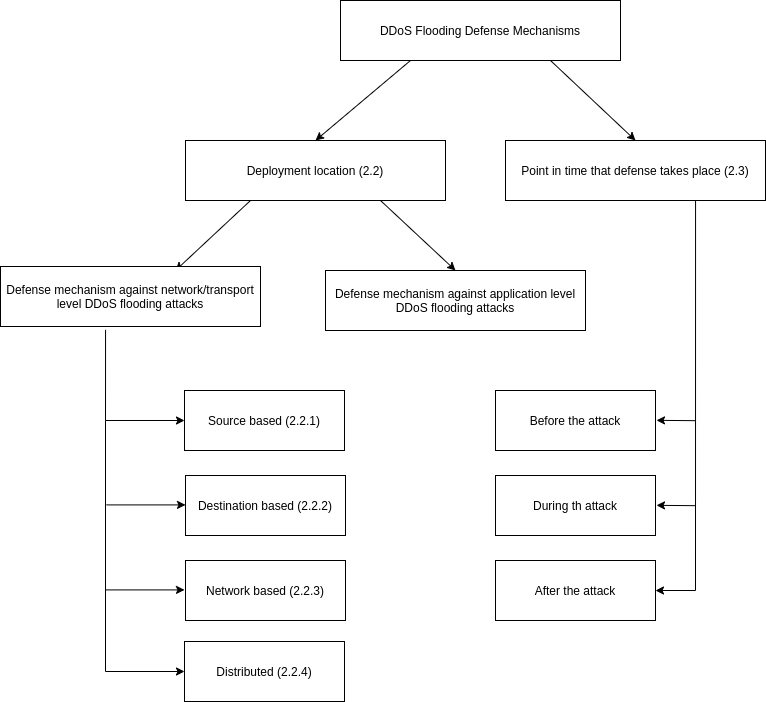
\includegraphics[width=\hsize]{images/ddos/ddos_flooding_defence.png}
    \caption{Meccanismi di difesa contro DDoS di tipo flooding.}
    \centering
\end{figure}

% \section{Tolleranza}
